\svnkwsave{$RepoFile: siminos/spatiotemp/chapter/reportAKS.tex $}
\svnidlong {$HeadURL: svn://zero.physics.gatech.edu/siminos/spatiotemp/chapter/reportAKS.tex $}
{$LastChangedDate: 2020-05-07 17:34:06 -0400 (Thu, 07 May 2020) $}
{$LastChangedRevision: 7184 $} {$LastChangedBy: predrag $}
\svnid{$Id: reportAKS.tex 7184 2019-12-12 06:24:59Z predrag $}

\chapter{Symbolic Dynamics for Coupled Cat Maps}
\label{chap:reportAKS}

\noindent
{\Large{\textbf{Adrien K. Saremi Summer 2016 Report}}}

\medskip

\noindent
{\large{\bf Abstract}}
\\
Classical particles are governed by Hamiltonian equations of motion.
Instead of continuous function of time, we break down our system's
evolution through a series of discrete instants; the generalized
coordinates $\{q_{n,t}, p_{n,t} \}$ are then solutions to a system of
coupled linear equations, written down in matrix form. Our research
consists in studying symbolical dynamics in relation with our
$N$-particle system, through a time evolution of length $T$ by obtaining
the nature of our alphabet, by computing the frequencies of appearance of
our symbols and by deriving the inadmissible symbolic spatiotemporal domains, through
analytic studies and computational models.

\section{Introduction}
\label{sect:introRepAKS}

Let a system of $N$ particle, evolving through time, over a time lapse of
value $T$. We assume that our system lies in one dimension of space,
therefore our generalized coordinates, position and momentum are
described as follows:
 \[
 \{q_{n,t}, p_{n,t}\} \: \text{where} \: n \in \{1, \dots, N\} \: \text{and} \: t \in \{1, \dots, T\}
 \]
Obviously, $n$ is the particle variable and $t$ the time variable. We also refer to $n$ as our space variable. At an instant $t$, we define our generalized coordinate vector $\mathcal{Z}_t$:

\[
\mathcal{Z}_t = \left \{
		\begin{array}{c}
		q_{n,t}\\
		p_{n,t}\\
		\end{array}
		\right \}_{1 \leqslant n \leqslant N}
		= \left \{
		\begin{array}{c}
		q_{1,t}\\
		p_{1,t}\\
		q_{2,t}\\
		p_{2,t}\\
		...\\
		p_{N,t}\\
		q_{N,t}\\
		\end{array}
		\right \}
\]
\\
Following Gutkin and Osipov\rf{GutOsi15}
{\em Classical foundations of many-particle quantum chaos},
we write Hamilton's equations for our generalized coordinate vector
$\mathcal{Z}_t$ described in this paper's sect.~\textit{3.1~Dynamics}:
 \[ \mathcal{Z}_{t+1} = \mathcal{B}_N \mathcal{Z}_t \]
with
\bea
\mathcal{B}_N &=& \left (
		\begin{array}{cccccc}
		A & B & 0 & \dots & 0 & B \\
		B & A & B & \dots & 0 & 0 \\
		0 & B & A  & \dots & 0 & 0 \\
		\vdots  & \vdots & \vdots & \ddots & \vdots & \vdots \\
		0 & 0 & 0 & \dots & A & B \\
		B & 0 & 0 & \dots & B & A \\
		\end{array}
		\right )
\continue
A &=&  \frac{1}{c} \left (
		\begin{array}{cc}
		a&1 \\
		ab - c^2&b \\
		\end{array}
		\right )
\,,\quad
B = -\,\frac{1}{c}  \left (
\begin{array}{cc}
d & 0 \\
db & 0 \\
\end{array}
\right )
\eea

We start with a system of just $N=1$ particle. This is usually referred
as \textit{Arnol'd cat map}.

\section{Arnol'd Cat Map}
\label{sect:AKSArnCat}

In this section, we introduce the concept of iterative process and
compute the time evolution of our system. We fix the parameters of
our $\mathcal{B}_N$ matrix:
\[ \mathcal{B}_N = \mathcal{B}_1 = A = \left (
\begin{array}{cc}
1 & 1 \\
1 & 2 \\
\end{array}
\right )
\,,\qquad
\det A= 1
\,.
\]
Here we picked the values $a=1$, $b=2$ and $c=-1$. The system of equations can be rewritten:
\beq
\left (
\begin{array}{c}
q_{t+1} \\
p_{t+1} \\
\end{array}
\right ) = A \left (
\begin{array}{c}
q_t \\
p_t \\
\end{array}
\right ) \mod\: 1
\ee{ASCatMap3}

For the sake of phase space volume conservation, we set the matrix $A$ to
have a determinant equal to $1$. The underlying difficulty of this
problem is that our coordinates must also remain within an interval of
length $1$. At first we pick this interval to be $[0,1)$. We will see
later that we change this interval to $[ -\frac{1}{2}, \frac{1}{2})$ in
order to preserve the symmetry of our coordinates and of our symbolic
dynamics with respect to $0$.

Our goal is now to find prime periodic orbits $p$ of period ${\cl{p}}$  and
initial points $\{q_{p,1},p_{p,1}\}$ such that:
\[ \left (
\begin{array}{c}
q_{p,{\cl{p}}} \\
p_{p,{\cl{p}}} \\
\end{array}
\right ) =
\left (
\begin{array}{c}
q_{p,1} \\
p_{p,1} \\
\end{array}
\right ) \mod\: 1
\]

In what follows, we explain the two approaches in order to reach this
goal. For the sake of notational simplicity, we denote our initial set as
$\{q_1, p_1\}$,and the final set as $\{q_{\cl{p}}, p_{\cl{p}}\}$. It
is understood that we deal with the prime periodic orbit $p$.

\subsection{\Po s - first approach}
\label{sect:AKS1stApp}

Consider
\[ \left (
\begin{array}{c}
q_{\cl{p}} \\
p_{\cl{p}} \\
\end{array}
\right ) = A^{\cl{p}} \left (
\begin{array}{c}
q_1 \\
p_1 \\
\end{array}
\right ) \mod\: 1 \]
We demand that $\{q_1,p_1\}$ is a periodic point in a prime periodic orbit
$p$ on a two--dimensional torus ${\mbox{\bf T}}^{2}$, \ie, a \rpo\ on
$\integers^2$, periodic up to a shift by integers $\{m_q,m_p\}$:
\[
\left (
\begin{array}{c}
q_1 \\
p_1 \\
\end{array}
\right ) = A^{\cl{p}}
\left (
\begin{array}{c}
q_1 \\
p_1 \\
\end{array}
\right ) + \left (
\begin{array}{c}
m_q \\
m_p \\
\end{array}
\right )
\]
Therefore:
\[
\left (
\begin{array}{c}
q_1 \\
p_1 \\
\end{array}
\right ) =
(\mathds{1} - A^{\cl{p}})
\left (
\begin{array}{c}
m_q \\
m_p \\
\end{array}
\right )
\]

The number of periodic orbits (AKA the number of sets of $\{q_1$,$p_1\}$0 would be then
given by:
\[
|\det(\mathds{1} - A^{\cl{p}})| = |(1-\lambda^{\cl{p}})(1-\frac{1}{\lambda^{\cl{p}}})|
\]
where $\lambda$ is the largest eigenvalue of $A$:
$\lambda = \frac{3 + \sqrt{5}}{2} = 2.6180$ also known as \textit{Floquet multiplier}
\vskip 0.2in
Instead of dealing with multiples of the $A$ matrix, and the large number
of coordinate vectors $\mathcal{Z}_t$, the second approach includes a
larger matrix computation, but allows us to store all coordinates in one
single vector.

\subsection{\Po s - second approach}
\label{sect:AKS2ndApp}

Here we eliminate $\{p_t\}$ in favor of a 2-step recurrence equation
on the position coordinate $\{q_t\}$:
\[
p_t = \frac{q_t - q_{t-1}}{\Delta t} = q_t - q_{t-1}
\]
Combined with:
\[
q_{t+1} = q_t + p_t
\]
We obtain:
\[
q_3 - 3q_2 + q_1 = m_2
\]
\[
q_4 - 3q_3 + q_2 = m_3
\]
\[\vdots\]
\[
q_{{\cl{p}}+1} -3q_{\cl{p}} + q_{{\cl{p}}-1} = m_{\cl{p}}
\]
\beq
q_{{\cl{p}}+2} -3q_{{\cl{p}}+1} + q_{\cl{p}} = m_{{\cl{p}}+1}
\ee{ASCatMap2a}
Since we look for periodic orbits,
$q_{{\cl{p}}+1} = q_1$ and $q_{{\cl{p}}+2} = q_2$.
Therefore the last equation reduces to:
\[
q_2 - 3q_1 + q_{\cl{p}} = m_1
\,,
\]
and the system of equations into the matrix form:
\[
\mathcal{D} \: Q_{\cl{p}}  =  m_{\cl{p}}
\]
with
\bea
Q_{\cl{p}} &=& \left (
\begin{array}{c}
q_1\\
q_2\\
\vdots \\
q_{\cl{p}}
\end{array}
\right )
            \,,\qquad
m_{\cl{p}} =  \left (
\begin{array}{c}
m_1\\
m_2\\
\vdots \\
m_{\cl{p}}
\end{array}
\right )
        \continue
\mathcal{D}  &=&  \left (
\begin{array}{ccccccc}
-3 & 1 & 0 & 0 & 0 & \dots & 1 \\
1 & -3 & 1 & 0 & 0 & \dots & 0 \\
\vdots & & & & & & \\
1 & 0 & 0 & 0 & \dots & 1 & -3 \\
\end{array}
\right )
\label{AKSdefD}
\eea

It then comes down to the nature of our initial set: if the starting set
is rational, we will necessarily obtain a periodic system. Indeed, if we
assume that the initial momentum and position are rational numbers with
some common denominator $N$, and since the cat map is composed of
integers, after $t$ steps, momentum and coordinate have the form $q_t =
a_t/N$, $p_t = b_t/N$. And if we travel on the lattice of the size
$N\times N$, it will take us a maximum step $N$ to close the loop.
Usually, the periodicity is smaller than $N$, and this is what our MATLAB
code computes.

\subsubsection{Program evaluation}


Using the 2$^{nd}$ approach, \refsect{sect:AKS2ndApp}, our program
computes the position coordinates of our particle for a given initial
condition $\{q_1, q_2\}$. The numbers $\{q_t\}$'s and the integers
$\{m_t\}$'s are then stored in the matrices $Q$ and $m$. The program
stops if for some iteration $t$ we obtain the same starting set
$\{q_{t+1}, q_{t+2}\} = \{q_1, q_2\}$, in which case the period is
${\cl{p}} = t$.

If it doesn't stop, and it completes all the iteration that the user
required, the program then looks for periodic behavior in the $m$ matrix.
In other words: does an integer ${\cl{p}}$ exist such that for all $t$,
$m_{t + {\cl{p}}} = m_t$. If it's the case, the orbit in question is
also periodic, and the program wasn't accurate enough to observe
periodicity among the position coordinates (a point that we will discuss
later this section).

\subsubsection{Results for \po s}

We now understand that the rational nature of our initial set $\{q_1, q_2\}$ is determinant for the periodic behavior of our system. We try several sets $\{q_1, q_2\}$ of the form $\{q_1, q_2\} = \{\frac{i}{N}, \frac{j}{N} \}$ where $i, j \in \{0, \dots, N-1\}$.

\begin {itemize}
\item
For $\{q_1, q_2\} = \{\frac{i}{10},\frac{j}{10}\}$, the periodicities found were: ${\cl{p}} = 1, 2, 3, 6, 10, 30$
\item
For $\{q_1, q_2\} = \{\frac{i}{100},\frac{j}{100}\}$, they were: ${\cl{p}} = 1, 2, 3, 6, 10, 30, 50, 150$
\item
For $\{q_1, q_2\} = \{\frac{i}{8},\frac{j}{8}\}$, ${\cl{p}} = 1, 3, 6$
\item
And for $\{q_1, q_2\} = \{\frac{i}{17},\frac{j}{17}\}$ ${\cl{p}} = 1, 18$
\item
Nevertheless, for an irrational starting set such as  $\{q_1, q_2\} = \{\frac{\pi}{6},\frac{\pi}{8}\}$ we do not obtain any periodic behaviors, despite running $20\,000$ iterations.
\end {itemize}

Before moving to the next part, we briefly discuss the accuracy of our computations, and the limits of our program when it comes to find periodic orbits.

\subsubsection{Round-off errors}

Our MATLAB calculations often gave us unexpected results, where we could
not find periodic orbits through our position coordinates. The advantage
of looking at the $m$ sequence instead is that it is made of integers,
while the $q$'s are decimal numbers, and it is possible that after many
iteration, the round-off error in computation becomes quite large.

In fact, such errors are directly related to the nature of our system, more
precisely the matrix $A$. The Floquet multiplier $\lambda$ has an impact
on the calculation of the computed value after $t$ iterations, compared
to the real value $q_{real,t}$:
\[
q_{computed,t} = q_{real,t} + \epsilon \: \lambda^{t} \text{, where } \lambda = \frac{3+\sqrt{5}}{2} = \text{multiplier}
\]
and where $\epsilon$ is the round off error of the system. For a 64-bit
operating system, $\epsilon  = 2^{-53} \approx 10^{-16}$. Now, if we look
for a computed value of $q$ within $10^{-4}$ of its real value, then the
maximum number of iteration $t_{max}$ is technically:
\[
|\epsilon \: \lambda^{t_{max}}| \leq 10^{-4}
\]
\[
\Rightarrow t_{max} \approx \ln(\lambda) \: \ln(\frac{10^{-4}}{\epsilon})
\]
\[
\Rightarrow t_{max} = 26
\]

The exponential growth in error imposes the use of different computation
techniques, or to application of the command
\textbf{digits($\mathbf{n}$)} which forces $n$ significant digits to any
computations.

Through our MATLAB program, we now focus on the nature of the alphabet
($m$ matrix), as well as the frequency of appearance of our symbols. The
big stuff....

\subsection{Symbolic dynamics for 1 particle}
\label{AKSalphabet1particle}

\subsubsection{Nature of our alphabet}
We recall that given our matrix $A$:
\[
q_{i-1} + q_{i+1} = 3q_i + m_i  \hskip 0.1in  \forall i
\]
In fact for a random matrix $A$ (as long as $det(A) = 1$), if we denote the trace of $A$ by $s = $trace($A$), then this equation is rewritten as:
\[
q_{i-1} + q_{i+1} = s \: q_i + m_i  \hskip 0.1in  \forall i
\]
Since the nature of $m_i$ only depends on $q_{i-1}$, $q_{i+1}$ and $q_i$,
consider a sequence of length 3: $\{q_1, q_2, q_3\}$ with the constraint
conditions on $q_i$'s:
\[
\begin{array}{c}
q_1 + q_3 = s \: q_2 + m \\ [3pt]
q_i \in [0,1) \hskip 0.05in \forall i
\end{array}
\]
Then:
\[
\begin {array} {c}
0 \leqslant q_1 < 1 \\
0 \leqslant q_3 < 1 \\
m \leqslant q_1 + q_3 < m + s \\
\end {array}
\]
The value of $s$ then becomes determinant to why only few symbols are
admissible. For example, for $s = 3$ we find that $m_t \in \{-2, -1, 0, 1\}$.


\subsubsection{Frequencies of symbols}
Using our program, we then compute the frequencies of each symbol for the case $s = 3$. By performing 1 iteration in time to obtain $q_3$ from $q_1$ and $q_2$ and by repeating with several different starting set, we obtain a good probability distribution of symbolic dynamics. We pick starting sets of the form $\{q_1, q_2\} = \{\frac{i}{200}, \frac{j}{200}\}$ where $i, j \in \{0,\dots, 199\}$ and obtain a distribution over $40\,000$ points:
\[
p_{-2} =0.16583, p_{-1} = 0.33335, p_{0} =0.33310, p_{1} = 0.16773
\]
In fact, if we plug the different values of $m$ in the system of equation above for $s = 3$, we obtain inequalities on $q_1$ and $q_3$. The admissible area in our lattice defined by $(q_1, q_3)$ is then the probability of obtaining the symbol $p_m$. For example for $m = -1$:
\[
\begin {array} {c}
0 \leqslant q_1 < 1 \\
0 \leqslant q_3 < 1 \\
-1 \leqslant q_1 + q_3 < 2 \\
\end {array}
\]
The admissible area is then $\mathcal{A} = 1$, but for $m = -2$:
\[
\begin {array} {c}
0 \leqslant q_1 < 1 \\
0 \leqslant q_3 < 1 \\
-2 \leqslant q_1 + q_3 < 1 \\
\end {array}
\]
And here the admissible area is $\mathcal{A} = \frac{1}{2}$. For $m = 0$ and $m = 1$, we respectively find $\mathcal{A} = 1$ and $\mathcal{A} = \frac{1}{2}$. Therefore our probability distribution matches our numerical calculations and:
\[
p_{-2} =\frac{1}{6}, p_{-1} =  \frac{1}{3}, p_{0} =\frac{1}{3}, p_{1} = \frac{1}{6}
\]
We observe that the inner symbols $-1$ and $0$ have a higher frequency than the outer ones, a point that will have a major importance when we study many symbols frequencies.

\subsubsection{Frequency of sequences of symbols}

\hskip 0.2in Another approach to the computation of one or more-than-two
sequence of symbols is to analyze the symbolic distribution over an
\textbf{ergodic} orbit, \ie, a non-periodic orbit. If the sequence of
symbols is long enough, one sequence is sufficient to observe a
frequency distribution that matches with the theory. This also works for
a given sequence of length $p$, such as $\{m_1 m_2 \dots m_p\}$. We
define $N_n(m_1 m_2, \dots m_p)$ as the number of periodic orbits of
length $n$ that generate the given sequence. The probability of obtaining
the sequence $\{m_1,m_2, \dots, m_p\}$ is then:
\[
p(m_1 m_2 \dots m_p) = \lim_{n\to\infty} \frac{N_n(m_1 m_2 \dots m_p)}{N_n}
\]

Figuring out the probability distribution by mathematical analysis (as we
did for 1 symbol) can become quite hard as the length of the given
sequence increases. We will cover in this section the case of many
particles. However, what we can observe is the correlation between
disjoint sequence of symbols.

Given a sequence $A = [a_1, \dots, a_u ]$ of length $u$, and a sequence
$B =  [a_1, \dots, a_v]$ of length $v$, we now examine the frequency of
seeing one repeated a length $space$ after the other. Comparing with the
product of their distinct frequencies, we then increase the
\textit{spacing} and observe how the correlation factor
\[
  Correl = p(A,space,B) - p(A) \: p(B) \: \text{behaves}
  \]
We obviously limit our study to admissible sequences. For the ergodic
orbit $ \{q_1,q_2\} = \{ \frac{\sqrt{5}}{4}, \frac{\sqrt{2}}{2} \} $ of
length $N = 1,000\,000$, and the sequences $A = [-1,1] $ and $B = [-2,0]$
\[
   p(A) = 0.1249 \hskip 0.2in p(B) = 0.0623
\]

   \[
\begin{array}{|c c c|}
\hline
Spacing & P(A,space,B) & Correl \\ [0.5ex]
\hline \hline
1 & 0.0085 & 7.3567\:10^{-4} \\
\hline
2 & 0.0066 & -0.0011\\
\hline
3 & 0.0073 & -4.6733\:10^{-4}\\
\hline
4 & 0.0080 & 1.8867\:10^{-4}\\
\hline
5 & 0.0079 & 6.8666\:10^{-5}\\
\hline
6 & 0.0078 & 4.6655\:10^{-6}\\
\hline
\end{array}
\]

For longer sets $A = [-1,-1,-1,-1]$ and $B = [-2,1,-1,0]$, and the same
orbit, the probabilities are as follow:
\[
   p(A) = 0.0178 \hskip 0.2in p(B) = 0.0151
\]

\[
\begin{array}{|c c c|}
\hline
Spacing & P(A,space,B) & Correl \\ [0.5ex]
\hline \hline
1 & 2.9400\:10^{-4} & 2.4439\:10^{-5}\\
\hline
2 & 2.2400\:10^{-4} & -4.5561\:10^{-5}\\
\hline
3 & 2.4900\:10^{-4} & -2.0561\:10^{-5}\\
\hline
4 & 2.5100\:10^{-4} & -1.8561\:10^{-5}\\
\hline
5 & 2.7300\:10^{-4} & 3.4392\:10^{-6}\\
\hline
6 & 2.6900\:10^{-4} & -5.6081\:10^{-7}\\
\hline
\end{array}
\]
\vskip 0.05in
In both scenarios, the correlation factor diminishes as the separation between the two blocs increases.  We notice that for longer sets $A$ and $B$, the correlation is small enough (but not zero) even for small spacing. It is quite interesting how this correlation, which translates the dependence between future and past symbolic dynamics, vanishes exponentially...

%%%%%%%%%%%%%%%%%%%%%%%%%

\section{Coupled Cat Maps}

\hskip 0.2in We now extend our study to a many particle system, where $N$
is the number of particles. $T$ will be now known as the period of the
orbit, and if it doesn't exist, $T$ will just refer to our ultimate time
iteration in the computation of the symbols $m$'s. Among the objectives
of this section, we will explain the impact of the trace of the $A$
matrix ($s = $trace$(A)$) on the nature of our alphabet, the length of
the periodic orbits, and the admissibility of sequences of symbols.

We will first look at the computation of our periodic orbits, then the
nature of our alphabet, and finally the rules that determine whether a
sequence of symbols is inadmissible, and if not, what is its frequency of
recurrence.

\subsection{Computation of symbols}

As we saw in \refsect{sect:AKSArnCat}, there are two approaches to
compute our symbolic dynamics. Here the 1st method that we described in
\refsect{sect:AKS1stApp} presents more advantage in the computation of
another symbolic dynamics.

\subsubsection{Computing the coordinates}

Our interval of study is $[-\frac{1}{2}, \frac{1}{2})$, the equation
$\mathcal{Z}_{t+1} = \mathcal{B}_N \: \mathcal{Z}_{t} \mod 1$ involves
the introduction of \textit{generalized} symbolics $m^{q,p}$ such that:
\[
\mathcal{Z}_{t+1} = \mathcal{B}_N \: \mathcal{Z}_{t} + m^{q,p}_{t+1}
\]
\[
\text{where  } m^{q,p}_t = \{m^q_t, m^p_t\} = \{m^q_{1,t}, m^p_{1,t}, m^q_{2,t}, m^p_{2,t}, \dots, m^q_{N,t}, m^p_{N,t}\}
\]
In fact the MATLAB can now store all the entries of the $\mathcal{Z}_t$
vectors in a larger matrix, where $T$ is the number of columns, and $2N$,
which refers to the 2 coordinates or each particle, is the number of
rows.

In a effort to keep the time evolution row-wise, and the space evolution
column-wise, only the momentum coordinates $\{q_{n,t}\}^{1\leqslant n
\leqslant N}_{1 \leqslant t \leqslant T}$ are then stored in the $Q$
matrix:
\[
Q = \left( \begin{array}{c}
q_{n,1} \\
q_{n,2} \\
\vdots \\
q_{n,T}
\end{array} \right)
=
\left( \begin{array}{cccc}
q_{1,t} & q_{2,t} & \dots & q_{N,t}
\end{array} \right)
=
\left( \begin{array}{cccc}
q_{1,1} & q_{2,1} & \dots & q_{N,1} \\
q_{1,2} & q_{2,2} & \dots & q_{N,1} \\
\vdots & \vdots  & \: & \vdots \\
q_{1,T} & q_{2,T} & \dots & q_{N,T} \\
\end{array} \right)
\]
Note that in the label $Q = \{q_{n,t}\}$, the column index is $n$ and
the row index is $t$.

\subsubsection{Computing the alphabet}

What we actually focus on is the symbolic dynamics. The $m^{q,p}$ matrix
mentioned above is the \textit{generalized} dynamics, while the one we
studied for $N = 1$ was the \textit{Newtonian} dynamics $m$. There are
two ways to compute the later:
\begin{itemize}
\item
Use our generalized symbolics:
\[
m_{n,t} = -b \: m^q_{n,t} - c \: m^q_{n,t+1} + m^p_{n,t}
\]

\item
Use the $Q$ coordinates:
\[
c\:(q_{n,t+1} + q_{n,t-1}) + d\:(q_{n+1,t} + q_{n-1,t}) = -s \: q_{n,t} + m_{n,t}
\]
\end{itemize}

For computations of admissible sequences, the later method is preferred.
And even if our dynamics is not defined at the boundaries, for either $n
\in \{1, N\}$ or $t =\in \{1, T\}$, the choice of ergodic orbits that run
for very large $N$ and $T$ makes irrelevant that a few number of symbols
can no longer be computed. For the case of periodic orbits, where $T$ is
usually a small number, we will only focus on the generalized coordinates
$m^{q,p}$ instead.

\subsubsection{\Po s}

The absolute criteria to obtain periodic orbits is to start with a
rational set $\mathcal{Z}_1$, and use integers for the parameters $a, b,
c$ and $d$. Unless specified, we use the following values throughout the
rest of our study:

\begin{itemize}
\item
$c = -1$ such that $det(A) = 1$
\item
$d = c$ in order to preserve the symmetry between space and time evolutions
\item
$b = 1$ and $a = 2$ in order to obtain $s = a+b = $trace$(A) = 3$. To observe a hyperbolic evolution, $a$ must remain greater than $2$; which is why we will only increase the value of $a$, and leave $b$ as a fixed parameter, to study the influence of $s$ on our system.
\end{itemize}
Few periodic orbits were computed, for different number of particles:

\begin{itemize}

\item
$
\text{for} \: N = 3 \: \text{and} \: \mathcal{Z}_1 = \left\{ \begin{array}{cccccc} \frac{31}{100} & \frac{29}{100} & \frac{7}{50} & - \frac{13}{100} & \frac{31}{100} & \frac{3}{100} \end{array}\right\}
$
\vskip 0.1in
the periodicity is $T = 60$, and the symbolic dynamics is:
\[
\begin{array}{c}
m^{q,p} = -2, p_{-2} = 0.011111 \\
m^{q,p} = -1, p_{-1} = 0.222222 \\
m^{q,p} = 0, p_{0} = 0.536111 \\
m^{q,p} = 1, p_{1} = 0.227778 \\
m^{q,p} = 2, p_{2} = 0.002778\\
\end{array}
\]

\item
for $N = 7$ and
{ \small
\[
\mathcal{Z}_1 =
\left\{
\frac{-19}{100} ~ \frac{21}{50} ~
\frac{-7}{100} ~ \frac{-8}{25} ~ \frac{2}{5} ~ \frac{47}{100} ~
\frac{-7}{100} ~ \frac{-39}{100} ~ -\frac{1}{4} ~ -\frac{1}{10} ~
\frac{9}{100} ~ \frac{-6}{25} ~ \frac{1}{10} ~ \frac{21}{100}
\right\}
\]
} %end  \small


the periodicity is $T = 2790$, and the symbolic dynamics is:
\[
\begin{array}{c}
m^{q,p} = -2, p_{-2} = 0.012110 \\
m^{q,p} = -1, p_{-1} = 0.226472 \\
m ^{q,p} = 0, p_{0} = 0.526882 \\
m^{q,p} = 1, p_{1} = 0.224014 \\
m^{q,p} = 2, p_{2} = 0.010522 \\
\end{array}
\]

\end{itemize}
By always finding periodicity, the program confirms that it evaluates the
right coordinates. It also validate that neither the number of particle
$N$, nor the periodicity $T$ have an influence on the nature of our
alphabet.


\subsection{Nature of our alphabet}
\label{AKSalphabet}

Through an analytic study, and by confirm with our simulations, we now
focus on the impact of the trace of A

\subsubsection{Analytically}

Given equation ???? and with $c = d = -1$:
\[
 s \: q_{n,t} = q_{n,t+1} + q_{n,t-1} + q_{n+1,t} + q_{n-1,t} + m_{n,t}
\]
Since we study the nature of 1 symbol at the time, let's pick the following notations
\[
n = 1 \: \text{and} \: t = 1
\]
\[
q_{1,1} = q_1 \hskip 0.2in m_{1,1} = m_1 \hskip 0.2in q_{1,0} = x_1 \hskip 0.2in q_{2,1} = x_2 \hskip 0.2in q_{1,2} = x_3 \hskip 0.2in q_{0,1} = x_4
\]
A system is relabelled as (we will see that this
notation is useful for sequence of many symbols)
\[
\begin{array}{ccc}
\: & q_{1,0}& \: \\
q_{0,1}& \boldsymbol{q_{1,1}} & q_{2,1}\\
\: & q_{1,2}& \:
\end{array}
\;=\;
\begin{array}{ccc}
\: & x_1 & \: \\
x_4 & \boldsymbol{q_1} & x_2 \\
\: & x_3 & \:
\end{array}
\,.
\]
This system we can rewrite as:
\[
q_1 = \frac{1}{s} (m_1 + \sum_{i = 1} ^ {4} x_i)
\]
with the constraints on $q_1$ and $x_i$:
\[
\left\{
\begin {array} {l}
-\frac{s}{2} \leqslant m_1 +  \sum\limits_{i = 1} ^ {4} x_i < \frac{s}{2} \\
-\frac{1}{2} \leqslant x_i < \frac{1}{2}
\,,\qquad\qquad
\text{ for } i = 1, \dots, 4
\end {array}
\right.
\]
For the Arnol'd cat map case $s = 3$, this reduces to
\[
\left\{
\begin {array} {l}
-\frac{3}{2} - m_1 \leqslant \sum\limits_{i = 1} ^ {4} x_i \leqslant \frac{3}{2} - m_1\\
-2 \leqslant \sum\limits_{i = 1} ^ {4} x_i\leqslant 2
\end {array}
\right.
\]
This system of inequalities allows us to derive which symbols are
admissible. For a given $m_1$, the system doesn't admit real solutions for
$x_i$'s (or if the solution is empty), then the symbol is forbidden. For
the case $s = 3$, we confirm what we obtained for $N = 1$ and $m \in
\{-3, -2, \dots, 2, 3\}$.

\subsubsection{Program}

Here ergodic orbits run for a large number of particles and over many
time iterations $T$. To speed up the computing process, the program stops
looking for periodic orbits and only focus on the symbolic dynamics, as
well as it probability distribution. The simulations are for different
values of $s$, with $N = 5$, $T = 80\,000$, and a random irrational
starting set:
\[
\begin{array}{| ll | ll | ll |}
\hline
\multicolumn{2}{|c|}{s = 3} & \multicolumn{2}{c|}{s = 4} & \multicolumn{2}{c|}{s=5} \\
\hline
\: & \: & \: & \: & m = -4 & p_{-4} = 0.000592 \\
m = -3 & p_{-3} = 0.000850 & m = -3 & p_{-3} = 0.010696 &  m = -3 & p_{-3} = 0.040080 \\
m = -2 & p_{-2} = 0.067293 & m = -2 & p_{-2} = 0.126391 &  m = -2 & p_{-2} = 0.159941\ \\
m = -1 & p_{-1} = 0.264819 & m = -1 & p_{-1} = 0.236452 & m = -1 & p_{-1} = 0.198742\\
m = 0 & p_{0} = 0.332571 & m = 0 & p_{0} = 0.250635 & m = 0 & p_{0} = 0.199551 \\
m = 1 & p_{1} = 0.267269 & m = 1 & p_{1} = 0.239835 & m = 1 & p_{1} = 0.201197\\
m = 2 & p_{2} = 0.066364 & m = 2 & p_{2} = 0.125378 & m = 2 & p_{2} = 0.159721\\
m = 3 & p_{3} = 0.000833 & m = 3 & p_{3} = 0.010613 & m = 3 & p_{3} = 0.039697\\
\: & \: & \: & \: & m = 4 & p_{4} = 0.000479 \\
\hline
\end{array}
\]
\[
\begin{array}{| ll | ll |}
\hline
\multicolumn{2}{|c|}{s = 6} & \multicolumn{2}{c|}{s = 7} \\
\hline
\: & \: & m = -5 & p_{-5} = 0.000363 \\
m = -4 & p_{-4} = 0.006921 & m = -4 & p_{-4} = 0.028955 \\
m = -3 & p_{-3} = 0.083823 & m = -3 & p_{-3} = 0.113895\ \\
m = -2 & p_{-2} = 0.159604 & m = -2 & p_{-2} = 0.141662\\
m = -1 & p_{-1} = 0.167262 & m = -1 & p_{-1} = 0.142537  \\
m = 0 & p_{0} = 0.165642 & m = 0 & p_{0} = 0.144154 \\
m = 1 & p_{1} = 0.166942 & m = 1 & p_{1} = 0.142207\\
m = 2 & p_{2} = 0.159625 & m = 2 & p_{2} = 0.142849\\
m = 3 & p_{3} = 0.083206 & m = 3 & p_{3} = 0.114120\\
m = 4 & p_{4} = 0.006975 & m = 4 & p_{4} = 0.028863\\
\: & \: & m = 5 & p_{5} = 0.000396 \\
\hline
\end{array}
\]

The resulting alphabet increases in size for larger $s$. And the more
``centered" a symbol is, the more frequently it appears.

For $s \geqslant 3$, the number of different admissible symbols $L$ is
always greater than $7$. We define the \textit{external} symbols as the
$6$ outer symbols in our alphabet ($3$ on each side) and the
\textit{internal} symbols as the remaining ones. Then, for a given $s$,
the probabilities of the internal symbols tend to be the same, an
observation we will extend for sequences of many symbols.


\subsection{Admissibility of sequences of more than 2 symbols}

Knowing which symbols are admissible allows us to expand our study to
sequences of many symbols, spread over both space and time
dimensions. Consider sequence $m$:
\[
\left [
\begin{array}{ccc}
m_{1,1} & \dots & m_{j,1} \\
\vdots & \: & \vdots \\
m_{1,i} & \dots & m_{j,i}
\end{array}
\right ]
\text{ with } i \text{ and } j \geqslant 2
\]

\subsubsection{$[2\!\times\!2]$ spatiotemporal domains}

For aesthetic reasons, we redefine our symbols and our coordinates:
\[
\begin{array}{cccc}
\: & q_{1,0} = x_1 & q_{2,0} = x_2 & \: \\
q_{0,1} = x_8 & \boldsymbol{q_{1,1} = q_1} & \boldsymbol{q_{2,1} = q_2} & q_{3,1} = x_3 \\
q_{0,2} = x_7 & \boldsymbol{q_{1,2} = q_3} & \boldsymbol{q_{2,2} = q_4} & q_{3,2} = x_4 \\
\: & q_{1,3} = x_6 & q_{2,3} = x_5 & \:
\end{array}
\]
as well as $m_{1,1} = a_1$, $m_{2,1} = a_1$, $m_{1,2} = a_3$ and $m_{2,2} = a_4$.
And using the Newtonian equation ????, the system of inequalities then becomes:
\[
\begin {array} {l}
q_1 = \frac{1}{s} (a_1 + q_2 + q_3 + x_1 + x_8) \\ [3pt]
q_2 = \frac{1}{s} (a_2 + q_1 + q_4 + x_2 + x_3) \\ [3pt]
q_3 = \frac{1}{s} (a_3 + q_1 + q_4 + x_6 + x_7) \\ [3pt]
q_4 = \frac{1}{s} (a_4 + q_2 + q_3 + x_4 + x_5)
\end {array}
\,,
\]
with conditions
\[
\begin {array} {l}
\forall i \in \{1,\dots, 4\}\,,\qquad -\frac{1}{2} \leqslant q_i < \frac{1}{2} \\ [3pt]
\forall j \in \{1, \dots, 8\}\,,\qquad -\frac{1}{2} \leqslant x_j < \frac{1}{2} \\ [3pt]
\forall k \in \{1,\dots, 4\}\,,\qquad m_k \in \{\mbox{alphabet}\}
\end {array}
\]
\skip 0.15in
{For $s = 3$}:
\[
\begin {array} {l}
-\frac{3}{2} - a_1 \leqslant q_2 + q_3 + x_1 + x_8 < \frac{3}{2} - a_1\\ [3pt]
-\frac{3}{2} - a_2 \leqslant q_1 + q_4 + x_2 + x_3 < \frac{3}{2} - a_2\\ [3pt]
-\frac{3}{2} - a_3 \leqslant q_1 + q_4 + x_6 + x_7 < \frac{3}{2} - a_3\\ [3pt]
-\frac{3}{2} - a_4 \leqslant q_2 + q_3 + x_4 + x_5 < \frac{3}{2} - a_4
\end {array}
\text{    with   }
\left\{
\begin {array} {l}
-\frac{1}{2} \leqslant q_i < \frac{1}{2} \\ [3pt]
-\frac{1}{2} \leqslant x_j < \frac{1}{2} \\ [3pt]
m_k \in \{-3, -2, \dots, 2, 3\}
\end {array}
\right.
\]
For the Arnol'd cat map case $s = 3$, there are a total of $7^4 = 2\,401$
possible $[2\!\times\!2]$ spatiotemporal \brick s.
    \PC{2017-09-08 In \refref{GHJSC16} I wrote that the $d=1$
     Arnol'd cat map $s = 3$ alphabet has 5 letters
    $\A=\{\underline{2},\underline{1},0,1,2\}$. Am I wrong?
    You mean $d=2$ \catlatt\ $s = 3$ alphabet on
    $[-\frac{1}{2},\frac{1}{2})\times[-\frac{1}{2},\frac{1}{2})$
    phase space has $s+4=7$ letters?
    }
Running on Mupad, we
solve this system of inequalities for different $a$'s. The number of
empty solutions we obtain is 552 which represents a total of 23\%
inadmissible spatiotemporal domains, which seems too small...

\subsubsection{Running many sequences on MATLAB}

We now try to confirm this percentage using our MATLAB program. The
probabilistic distribution of every $[2\!\times\!2]$ spatiotemporal domain
has the  shape shown in \reffig{fig:AKS2x2all}.


\begin{figure}[h]
\centering
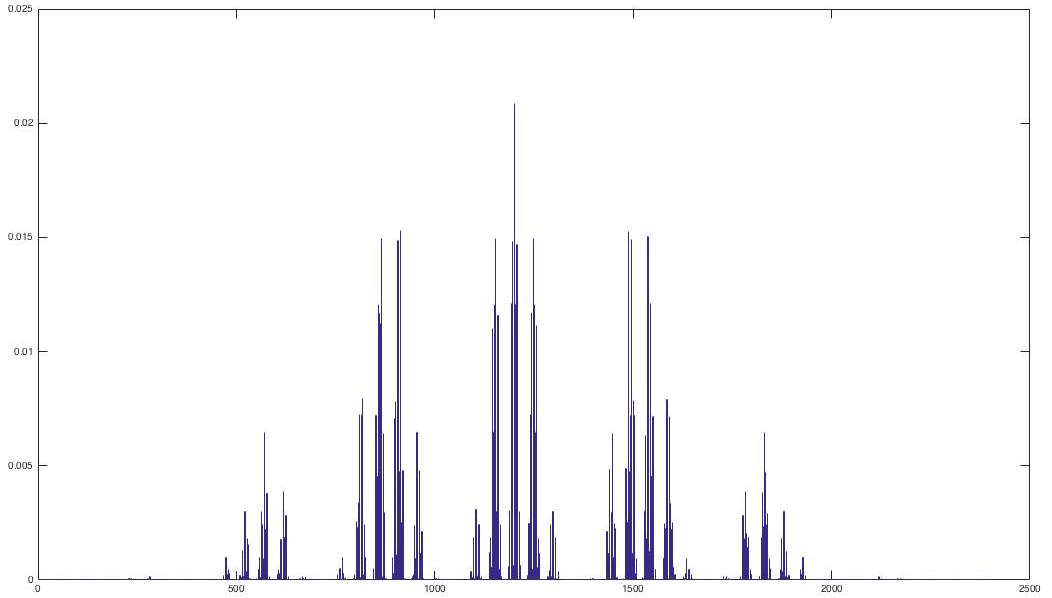
\includegraphics[width=\textwidth]{AKS2x2all}
\captionsetup{justification = centering}
\caption{\label{fig:AKS2x2all}
Probability distribution for {\em all} $[2\!\times\!2]$ spatiotemporal domains.
\\
$N =100 \hskip 0.1in T = 20\,000 \hskip 0.1in s = 3$.
        }
\end{figure}

The difference in results from our analytical study is quite significant
since the number of inadmissible sequences is 1,665 out of 2,401 (69.3\%). A
number that could be blamed on the size of our sample being not large enough.
Nevertheless, if our statistical analysis is improved, few other analysis can
be accomplished:

\begin{itemize}
\item
Try spatiotemporal domains of size $[3\!\times\!3]$. But because the
total number $7^9 = 40\,353\,607$, an even larger sample would then be
required to appropriately study the probability distribution of those
blocks, at least of order of $10^9$.
\item
Next, look for probing rules for spatiotemporal domains of size $[3\!\times\!3]$,
that are NOT probing rules for $[2\!\times\!2]$ spatiotemporal domains...
\end{itemize}

\subsubsection{Internal symbols}
We close our discussion by focusing on the significance or internal
symbols. The frequencies of appearance of all $[2\!\times\!2]$ and $[3\!\times\!3]$
internal blocks are analyzed for the case $s=5$. The internal symbols
are then $\{-1, 0, 1\}$ and the simulations are  for $N = 30$ and $T =
50\,000$. For this sample, the 81 $[2\!\times\!2]$ blocks of internal symbols
are spread evenly (figure 6.2 a), which confirms that for a given trace
$s$, the internal symbols have a uniform distribution. For the 19683 $[3\!\times\!3]$
blocks, the same behavior tends to be observed but the ratio
\textit{number of sequences} to \textit{size of the sample} seems once
again to ``deform" such distribution.

\begin{figure}[h]
\centering
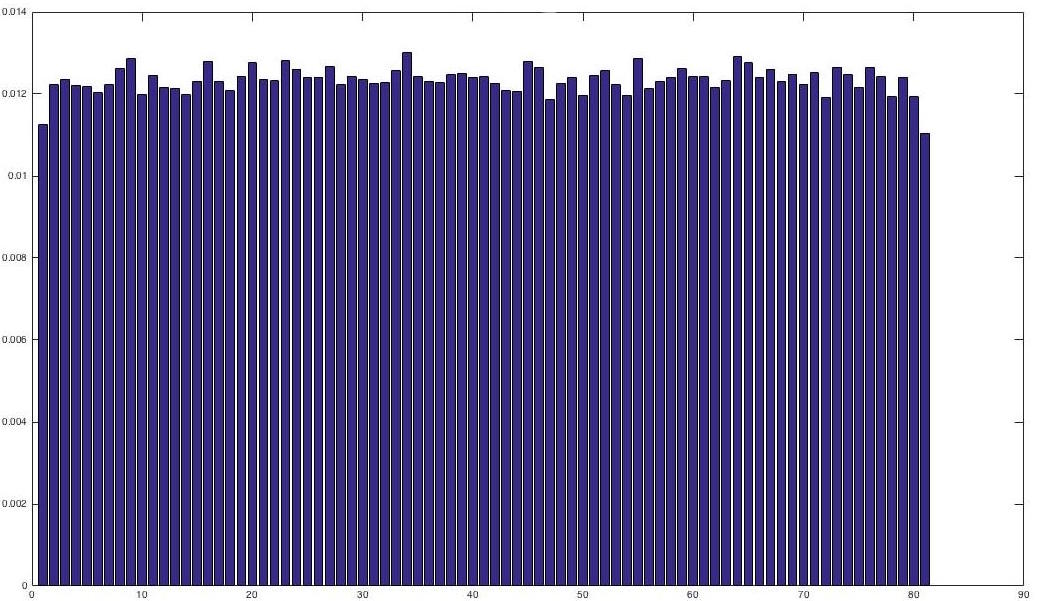
\includegraphics[width=\textwidth]{AKS2x2int}
\captionsetup{justification = centering}
\caption {\label{fig:AKS2x2int}
(a) $[2\!\times\!2]$ spatiotemporal domains.
    }
\end{figure}

\begin{figure}[h]
\ContinuedFloat
\centering
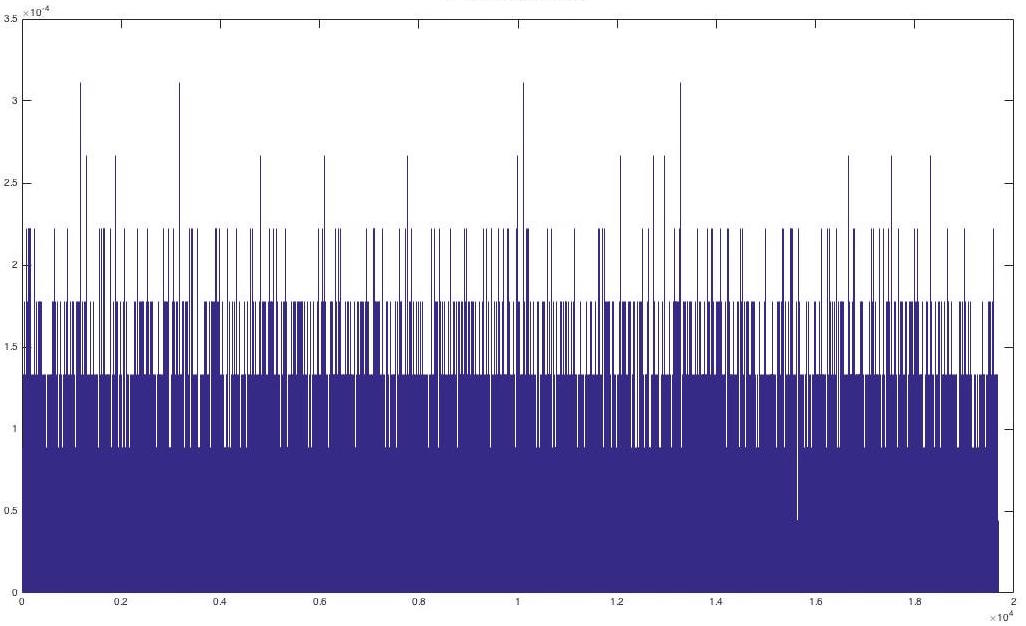
\includegraphics[width=\textwidth]{AKS3x3int}
\captionsetup{justification = centering}
\caption{\label{fig:AKS3x3int}
(b) $[3\!\times\!3]$ spatiotemporal domains.
\\ Probability distribution for sequences of internal symbols.
\\ $N =30 \hskip 0.1in T = 50\,000 \hskip 0.1in s=5$.
}
\end{figure}

\section{Future work...}

A lot still remains to be done in order to get a complete understanding
of Coupled Cat Maps. Among other things, one important factor is the fact
that this symbolic dynamics present a symmetry between space and time. In
\reffig{fig:AKS2x1all} the probability distribution for spatiotemporal domains of
shape $[2\!\times\!1]$ (evolution in time) and $[1\!\times\!2]$ (evolution in
space) are both drawn. A total of $81$ spatiotemporal domains in each case is
obtained, and present very similar distributions.
    \PC{2016-08-02 Rather than `similar', aren't they supposed to be identically
    the same? Are there some numerical differences in the columns of the two figures
    (they cannot be seen in the plots)?}

\begin{figure}[ht]
\centering
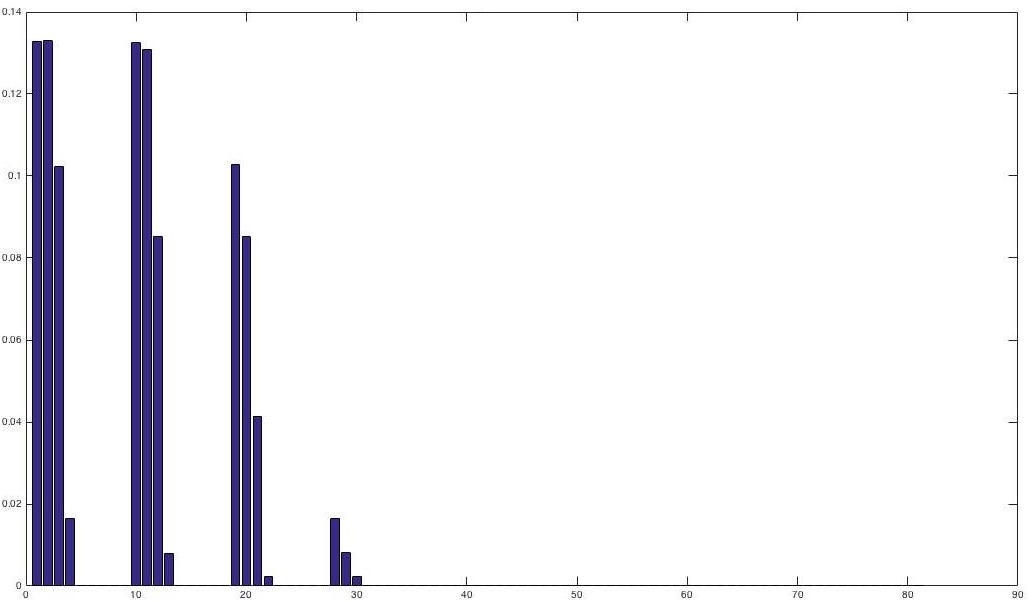
\includegraphics[width=\textwidth]{AKS2x1all}
\captionsetup{justification = centering}
\caption{\label{fig:AKS2x1all}
(a) $[2\!\times\!1]$ spatiotemporal domains.
        }
\end{figure}

Other future work also involve the reconstruction of orbits in the phase
space based on symbolic sequences. A significant step in the
understanding of semi-classical particles in a chaotic regimes...

\begin{figure}[ht]
\ContinuedFloat
\centering
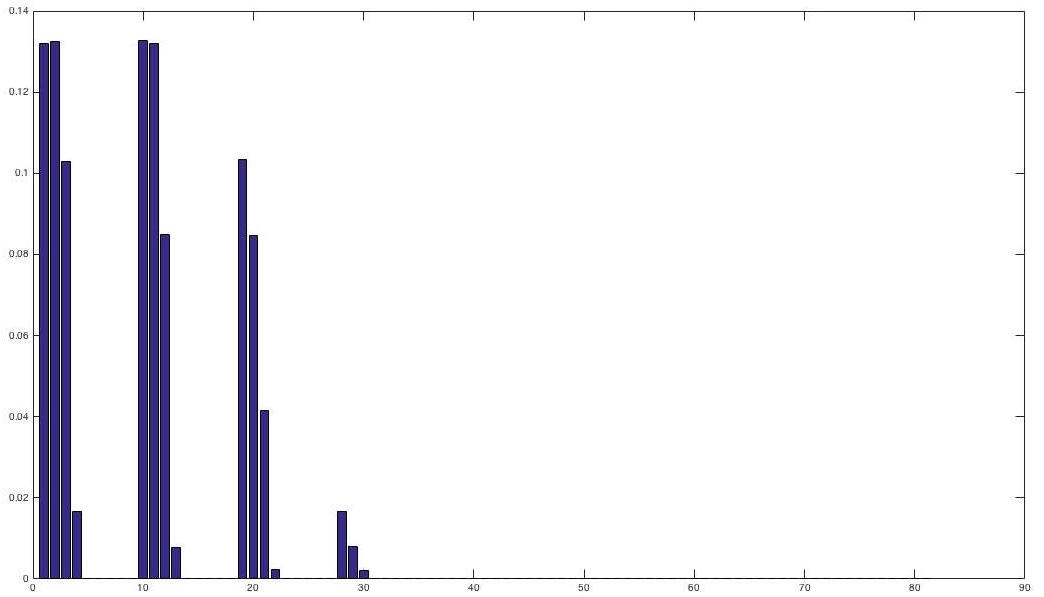
\includegraphics[width=\textwidth]{AKS1x2all}
\captionsetup{justification = centering}
    \caption{\label{fig:AKS1x2al1}
(b) $[1\!\times\!2]$ spatiotemporal domains. \\
Probability distribution of {\em all} $[2\!\times\!1]$ and $[1\!\times\!2]$
spatiotemporal domains.
$N =30 \hskip 0.1in T = 50\,000  \hskip 0.1in s=5$.
             }
\end{figure}



%%%%%%%%%%%%%%%%%%%%%%%%%%%%%%%%%%%%%%%%%%%%%%%%%%%%%%%%%%%%%%%%%%%%%%%
\printbibliography[heading=subbibintoc,title={References}]
